%%%%%%%% ICML 2025 EXAMPLE LATEX SUBMISSION FILE %%%%%%%%%%%%%%%%%

\documentclass{article}

% Recommended, but optional, packages for figures and better typesetting:
\usepackage{microtype}
\usepackage{graphicx}
\usepackage{subfigure}
\usepackage{booktabs} % for professional tables
\usepackage{float}

% hyperref makes hyperlinks in the resulting PDF.
% If your build breaks (sometimes temporarily if a hyperlink spans a page)
% please comment out the following usepackage line and replace
% \usepackage{icml2025} with \usepackage[nohyperref]{icml2025} above.
\usepackage{hyperref}

\usepackage{xurl}

% Attempt to make hyperref and algorithmic work together better:
\newcommand{\theHalgorithm}{\arabic{algorithm}}

% Use the following line for the initial blind version submitted for review:
%\usepackage{icml2025}

% If accepted, instead use the following line for the camera-ready submission:
\usepackage[accepted]{packages/icml2025}

% For theorems and such
\usepackage{amsmath}
\usepackage{amssymb}
\usepackage{mathtools}
\usepackage{amsthm}

% if you use cleveref..
\usepackage[capitalize,noabbrev]{cleveref}

% Configure cleveref names for appendix sections
\crefname{appendix}{Appendix}{Appendices}
\Crefname{appendix}{Appendix}{Appendices}

%%%%%%%%%%%%%%%%%%%%%%%%%%%%%%%%
% THEOREMS
%%%%%%%%%%%%%%%%%%%%%%%%%%%%%%%%
\theoremstyle{plain}
\newtheorem{theorem}{Theorem}[section]
\newtheorem{proposition}[theorem]{Proposition}
\newtheorem{lemma}[theorem]{Lemma}
\newtheorem{corollary}[theorem]{Corollary}
\theoremstyle{definition}
\newtheorem{definition}[theorem]{Definition}
\newtheorem{assumption}[theorem]{Assumption}
\theoremstyle{remark}
\newtheorem{remark}[theorem]{Remark}

% Todonotes is useful during development; simply uncomment the next line
%    and comment out the line below the next line to turn off comments
%\usepackage[disable,textsize=tiny]{todonotes}
\usepackage[textsize=tiny]{todonotes}

% The \icmltitle you define below is probably too long as a header.
% Therefore, a short form for the running title is supplied here:
\icmltitlerunning{Submission and Formatting Instructions for ICML 2025}

\begin{document}

\twocolumn[
  \icmltitle{Access Controls Will Solve the Dual-Use Dilemma}

  % It is OKAY to include author information, even for blind
  % submissions: the style file will automatically remove it for you
  % unless you've provided the [accepted] option to the icml2025
  % package.

  % List of affiliations: The first argument should be a (short)
  % identifier you will use later to specify author affiliations
  % Academic affiliations should list Department, University, City,
  % Region, Country
  % Industry affiliations should list Company, City, Region, Country

  % You can specify symbols, otherwise they are numbered in order.
  % Ideally, you should not use this facility. Affiliations will be numbered
  % in order of appearance and this is the preferred way.
  \icmlsetsymbol{equal}{*}

  \begin{icmlauthorlist}
    \icmlauthor{Evžen Wybitul}{eth}
  \end{icmlauthorlist}

  \icmlaffiliation{eth}{ETH Zurich, Switzerland}

  \icmlcorrespondingauthor{Evžen Wybitul}{wybitul.evzen@gmail.com}

  % You may provide any keywords that you
  % find helpful for describing your paper; these are used to populate
  % the "keywords" metadata in the PDF but will not be shown in the document
  \icmlkeywords{Gradient Routing, Modularization, AI Safety,
  Unlearning, Access Control, Technical AI Governance}

  \vskip 0.3in
]

% this must go after the closing bracket ] following \twocolumn[ ...

% This command actually creates the footnote in the first column
% listing the affiliations and the copyright notice.
% The command takes one argument, which is text to display at the
% start of the footnote.
% The \icmlEqualContribution command is standard text for equal contribution.
% Remove it (just {}) if you do not need this facility.

%\printAffiliationsAndNotice{}  % leave blank if no need to mention
% equal contributiono
\printAffiliationsAndNotice{} % otherwise use the standard text.

\begin{abstract}
  AI safety systems face the dual-use dilemma: it can be unclear whether to refuse certain requests, since they could be either harmless or harmful depending on who made them and why.
  The only way to know is to look at their real-world context, but current safety systems do not capture this information.
  Instead, they make arbitrary decisions that end up hurting both utility and safety: they sometimes refuse legitimate queries and sometimes fail to refuse harmful ones.
  To address this, we propose a conceptual framework based on access controls in which only verified users can access dual-use outputs.
  We describe the framework's components, analyse its feasibility, and explain how it addresses both over-refusals and under-refusals.
  While only a high-level proposal, our work makes the first step toward enabling granular AI governance that transforms traditional utility-safety tradeoff: users would gain access to more capabilities without sacrificing safety, and regulators would achieve better oversight without stifling innovation.
\end{abstract}

\section{Introduction} \label{section:introduction}

\emph{What features of viral surface proteins are recognized by human
antibodies?}

Is this question safe to answer?
While some user requests and large language model outputs are clearly benign or clearly harmful, many fall in the grey zone in the middle, as illustrated in \cref{figure:main}.
In the grey zone, the harmfulness of a request depends not on its content, but on its \emph{real-world context}: who made it and for what purpose.

\begin{figure}[t]
  \vskip 0.2in
  \begin{center}
    \centerline{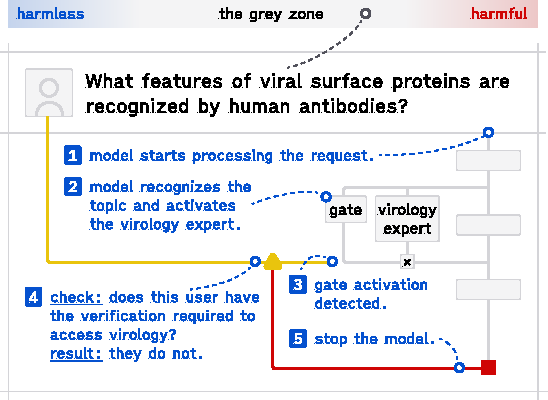
\includegraphics[width=\columnwidth]{assets/main_figure.pdf}}
    \caption{
      The user is asking a question from the grey zone: a question that could be either harmless or harmful, depending on its real-world context.
      The schema shows how the access control system we propose would handle it.
      (1)~The model begins to answer the question because it is trained to be helpful.
      (2)~During the forward pass, the model detects the question is about virology and activates its virology expert module that contains knowledge specific to that topic.
      (3)~The activation of the expert is observed by an external mechanism that immediately (4)~checks in the company's database if the user has the required authorization to access virology knowledge.
      (5)~Since they don't, the model is stopped.
    If they did, the model would be allowed to give an answer.}
    \label{figure:main}
  \end{center}
  \vskip -0.2in
\end{figure}

Safety systems that rely solely on content immediately face the \emph{dual-use dilemma}.
When confronted with a grey-zone request, should they refuse it or not?
This forces arbitrary decisions that reduce both utility and safety: some legitimate queries are refused (over-refusals) while some harmful ones are not (under-refusals).
Some safety systems attempt to address this by inferring the context of the request from its contents or the chat history.
However, this context is fully user-supplied and can be easily fabricated by adversaries.

In this paper, we argue that informative, hard-to-fabricate real-world context can be obtained through user-level verifications such as ID checks, institutional affiliations, or government-issued certifications.
We address the dual-use dilemma with two contributions.
\textbf{As our primary contribution}, we show how this verified context can be used jointly with content analysis in a safety framework based on access controls \cite{butler1974}.
In the framework, model outputs are classified into content categories, and the system verifies whether the user has the required credentials to access the detected category.
We also describe how the framework addresses both issues caused by the dual-use dilemma: over-refusals and under-refusals.
\textbf{Additionally}, we propose a novel theoretical approach to content category classification based on recent methods for robust unlearning, UNDO \cite{lee2025distillationrobustifiesunlearning} and gradient routing \cite{cloud2024gradientroutingmaskinggradients}.
This approach avoids the capability gap between a model and its monitors that can make output monitoring methods non-robust \cite{jin2024jailbreakinglargelanguagemodels}.

Our framework represents a first step toward solving the challenge of ``detection and authorization of dual-use capability at inference time'' highlighted by a recent survey of problems in technical AI governance \cite{reuel2025openproblemstechnicalai}.
Current regulatory approaches choose between blanket restrictions of capabilities that stifle innovation and blanket permissions that create safety risks.
Future implementations of such frameworks could instead enable granular policies that differentiate between types of users and their contexts.

\section{Current Safety Methods Don't Solve the Dual-Use Dilemma}
\label{section:current-methods}

The dual-use dilemma causes two issues: over-refusals and under-refusals.
Over-refusals reduce model utility for legitimate users, which is clearly undesirable.
Under-refusals are equally problematic because they enable decomposition attacks \cite{glukhov2023llmcensorshipmachinelearning, glukhov2024breachthousandleaksunsafe}.
These attacks transform clearly harmful queries, such as ``How to modify a virus to avoid immune detection?'', into series of mundane grey zone questions, such as ``What features of viral surface proteins are recognized by human antibodies?'' from \cref{figure:main}.
Safety systems would refuse the harmful query but do not refuse the grey zone questions since they are not individually harmful.
Through these attacks, adversaries exploit under-refusals to decrease system safety.

Since whether a grey zone request should be refused depends on who made it and why, preventing both over-refusals and under-refusals requires access to real-world context.
This means that the traditional focus on resilience against jailbreak and prompt injections is orthogonal to this problem.
Instead, we evaluate three approaches from the AI safety literature to see how sensitive they are to contextual information, and whether their sources of real-world context are trustworthy --- that is, hard to manipulate by an adversary.

\subsection{Unlearning: Non-Contextual Removal of Concepts}

Unlearning methods aim to remove specific knowledge, concepts, or
capabilities from a model after training
\cite{liu2024rethinkingmachineunlearninglarge}. Their goal is to
eliminate the model's ability to generate harmful content while
preserving other capabilities.

Unlearning faces significant technical challenges even for preventing behaviours that are clearly harmful.
As noted by \citet{cooper2024machineunlearningdoesntthink} and \citet{barez2025openproblemsmachineunlearning}, capabilities are hard to define, hard to remove without side effects, and hard to trace back to specific data points.
Furthermore, many unlearning approaches mask rather than truly remove the targeted knowledge \cite{deeb2025unlearningmethodsremoveinformation}.

\subsection{Safety Training: The Model Reacts to Context}

Safety training methods modify the model's training process to align
its outputs with human preferences.
This category includes safety pre-training \cite{maini2025safetypretraininggenerationsafe}, RLHF \cite{christiano2023deepreinforcementlearninghuman}, and safety finetuning.

Unlike unlearning, these methods are contextual.
They don't remove capabilities entirely but train the model to selectively deploy them based on, among other things, the perceived legitimacy and harmlessness of the request.
However, these qualities are entirely inferred from content supplied by the user, such as the request content or the chat history.
It should be no surprise, then, that models are susceptible to attacks that fabricate in-chat context \cite{zeng2024johnnypersuadellmsjailbreak}, or attacks that diminish models' sensitivity to in-chat context through multi-round escalation \cite{russinovich2025greatwritearticlethat}.
Without access to trustworthy real-world context of the request, the model cannot make truly informed decisions about grey zone requests.

\subsection{Post-Processing: External Systems React to Context} \label{section:post-processing}

Post-processing methods are systems that classify user inputs and model outputs for the purposes of steering the underlying model, or monitoring and filtering its outputs.
Sometimes, these methods are used for usage monitoring, as is the case with Anthropic's Clio \cite{tamkin2024clioprivacypreservinginsightsrealworld, handa2025economictasksperformedai}, other times, they are used for safety, as with Llama Guard \cite{inan2023llamaguardllmbasedinputoutput} and Constitutional Classifiers \cite{sharma2025constitutionalclassifiersdefendinguniversal}.
However, similarly to safety training, the ``real-world'' context these methods work with is currently inferred mostly from user-supplied content and thus untrustworthy and vulnerable to attacks, as evidenced by the many jailbreaks that successfully target current production systems \cite{zhang2025outputconstraintsattacksurface}.
Nevertheless, these methods could be modified to incorporate external contextual information, potentially serving as a foundation for more trustworthy, contextual safety mechanisms. We discuss this option in \cref{section:content-classification}.

\section{Access Controls as a Solution}
\label{section:access-controls}

Current safety systems face the dual-use dilemma because they lack trustworthy information about who is making a request and why.
In this section, we describe an access control system that addresses this problem by verifying user credentials before granting access to sensitive knowledge.

\subsection{Overview of the Access Control Framework} \label{section:access-control-overview}

We propose a defensive system where grey-zone requests are refused by default, but users can gain access to specific categories of knowledge if they undergo verification.

When model providers set up the system, they will make two design decisions with the help of domain experts.
First, they will define \textbf{content categories} (\cref{section:content-categories}): groups of sensitive topics organized by domain and risk rating.
Second, for each content category, they will specify a \textbf{verification mechanism} (\cref{section:verification-mechanisms}): the verification process users must complete to access that category.

Whenever the model generates an output, the system will perform \textbf{content classification} (\cref{section:content-classification}) to check whether the model's output belongs to any predefined content category.
If the user lacks authorization for the detected category, the system will implement appropriate \textbf{system responses} (\cref{section:system-responses}) ranging from enhanced logging to refusal.

For example, in biology, basic knowledge and common techniques would remain freely accessible, widespread techniques like CRISPR would likely only require ID-based verification, and dangerous techniques like aerosolization might require government biosafety certifications.
If a user asks for help with CRISPR laboratory protocols, the system would detect that the request belongs to a low-risk category, check whether the user has verified their ID, and either provide the information or prompt them to complete verification first.

This approach directly addresses both sides of the dual-use dilemma.
Decomposition attacks will become much harder because the system refuses grey-zone requests by default—attackers would need legitimate credentials rather than clever prompting.
Simultaneously, verified users will gain access to specialized knowledge that would otherwise face blanket restrictions under current approaches.

The main concern is increased user friction, but we argue in \cref{section:feasibility-and-limitations} that this will be minimal because most users will never make grey-zone requests.

\subsection{Content Categories} \label{section:content-categories}

Content categories are groups of sensitive topics organized by domain and risk level, which model providers will develop with domain experts.

We expect most implementations to follow a three-tier risk structure.
For example, in biology, common techniques would be classified as low-risk;
widespread techniques that pose some harm, such as CRISPR, would fall into a moderate-risk category;
and specialized techniques with limited legitimate uses, such as aerosolization of bacteria, would be classified as high-risk.

Experts could develop these categories by adapting existing risk frameworks, such as biosafety levels (BSL)~\cite{CDC_BMBL_2020} and dual-use research of concern policies~\cite{USG_DURC_2012} in biology.
However, since existing frameworks typically categorize only high-level concepts like organisms or compounds, experts would need to decompose them into smaller, more specific components.
For instance, cultivating and handling a dangerous BSL-3 pathogen might involve (1) specific procurement methods, (2) cultivation techniques, (3) purification methods, and (4) protocols for specialized equipment.
For each of these components, experts would assess the ratio of harmless to harmful applications it enables, then assign it to an appropriate (low, moderate, or high) risk category.

Evidence from chemistry suggests this approach could work: the risk schedules of the Chemical Weapons Convention already identify not just controlled compounds but also their precursors and specific equipment~\cite{OPCW_CWC_1993}, demonstrating successful decomposition into components.
Nevertheless, some harmful applications might not decompose so neatly; we discuss this limitation in \cref{section:feasibility-and-limitations}.

\subsection{Verification Mechanisms} \label{section:verification-mechanisms}

Each content category will have a verification process that users must complete to access it.
The system will initially vary across model providers, but we expect it to follow a three-tier structure, mirroring the risk structure of the content categories.
Most content will require no verification, moderate-risk content categories will require basic identity verification or institutional affiliation, and high-risk categories will require domain-specific certifications.
Rather than creating new systems, model providers will build on existing verification infrastructure, consulting domain experts to identify appropriate mechanisms for each field.

For low-risk content categories, model providers could use established identity verification services like Stripe Identity~\cite{stripe_identity_2024} or institutional systems like ORCID~\cite{orcid_2024}.
These systems provide global, standardized, low-friction solutions with one-time costs under \$2 per user.
They would serve primarily to maintain audit trails for post-incident investigation and provide a deterrent effect, rather than as security barriers for high-risk knowledge.

High-risk content categories could leverage existing domain-specific certifications that demonstrate users' ability to handle sensitive information and materials responsibly.
Model providers would work with domain experts and national authorities to identify appropriate certifications, adapting existing physical-world credential systems to knowledge access control.
For biological content categories, the system could draw on governmental certifications for handling high-BSL organisms, as mentioned in \cref{section:content-categories}, and equivalent certifications in other countries.

Governance of verification systems, including requirements and appeals processes, will initially vary across providers.
Over time, successful approaches may inform industry coordination and eventual standardization, similar to how content moderation and know-your-customer standards evolved.

This approach faces several limitations.
For high-risk categories, relying on existing certifications may be overly restrictive, potentially excluding some users who should have access.
However, we argue in \cref{section:feasibility-and-limitations} that knowledge in high-risk categories would likely face blanket restrictions anyway, and our approach enables access for verified users rather than complete prohibition.
In the same section, we discuss open problems including equity concerns regarding differential access for users in developing countries and privacy implications of credential verification systems.

\subsection{Implementing Content Classification} \label{section:content-classification}

Model providers will need to classify model outputs into content categories during generation.
We examine three possible implementations below.
While none of these approaches have been empirically validated for risk category classification specifically, each represents a plausible technical path that could be developed and evaluated by practitioners interested in implementing access controls.
We leave the discussion of how classification errors might influence user experience for \cref{section:feasibility-and-limitations}.

\paragraph{Separate Models}

The most straightforward approach is to create separate models with different capabilities, and route users to the appropriate model based on their authorization.

This approach offers strong robustness against adversarial attacks since unauthorized knowledge is physically absent from the model.
However, this approach proves impractical for real deployment, as model providers would need to train and maintain potentially dozens of model variants.

\paragraph{Specialized Expert Modules}

% TODO This approach offers a unique robustness property: if an adversary successfully prevents expert module activation to avoid detection, they simultaneously prevent access to the specialized knowledge stored in that module, making the attack self-defeating.

Instead of maintaining separate models, model providers could use a single model with separate expert modules that activate when their specialized knowledge is required.
\Cref{figure:main} illustrates this approach when a user asks about viral surface proteins.
When the model processes the request, it activates its virology expert module.
An external system observes this activation, checks the user's credentials, and decides whether to allow the model to deliver the response.
This method approximates the benefits of physically separated models while avoiding the overhead: a model provider trains one model but effectively gets multiple models in return.

To implement this, the model providers need a method that can take knowledge that starts out distributed throughout the model and concentrate it into the expert modules.
For this, we propose a method that is a combination of UNDO \cite{lee2025distillationrobustifiesunlearning} and gradient routing \cite{cloud2024gradientroutingmaskinggradients}.
The steps resemble the original UNDO: first, unlearn knowledge belonging to any content category from the model, then distil the unlearned model into a new model.
However, taking inspiration from the gradient routing paper, the new model would include expert modules for each content category, and during distillation, gradients from examples in the various content categories would be routed exclusively through their associated expert modules.
The model would also be explicitly trained to activate the expert modules only when generating content in their associated category.

This approach would offer several advantages.
First, it would add almost no latency since the expert modules are small, not activated very often, and there is no post-processing step.
Second, it could provide strong robustness: if an attacker prevents the activation of an expert module to avoid detection, the resulting output lacks the specialized knowledge.
Third, since the model is trained to activate the category-specific experts when they are needed, it should learn to recognize the content categories.
This stands in contrast to ex-post probing methods, which do not offer such guarantees.
While this method remains empirically unvalidated for our use case, the properties above make it worth investigating.

\paragraph{Post-Processing}

Post-processing methods such as Constitutional Classifiers \cite{sharma2025constitutionalclassifiersdefendinguniversal} offer a proven approach to content classification.
They operate independently of the model, allowing for rapid deployment and iteration, and they could be adapted to detect content categories and trigger checks of user verifications.
However, for latency reasons, there is sometimes a capability gap between the model and the post-processing system, which the adversaries can exploit to evade detection \cite{jin2024jailbreakinglargelanguagemodels, kumar2025freelunchguardrails}.

\subsection{System Responses} \label{section:system-responses}

If the user makes a request for content they are authorized to access, the system allows the model to generate the response.
Otherwise, the system responds in various ways based on the risk category and the confidence of the content classification.

For example, the initial implementation might use the following two response types:
First, outputs classified as belonging to restricted content categories with high confidence are immediately refused.
The system provides a message indicating which verification is required for access.
Second, if the classification is borderline, the model is allowed to continue generating the response.
However, the system turns on enhanced logging and conducts additional post-processing safety review before delivering the output to the user.

\section{Feasibility and Limitations}
\label{section:feasibility-and-limitations}

\cref{section:access-controls} identified several technical challenges in the access control system: (1)~some harmful knowledge might decompose into concepts that are all indispensable for harmless applications; (2)~some verifications may be too difficult to obtain; and (3)~content classifiers might produce false positives.
These challenges will increase user friction, imposing a cost on the utility of the system.
Prompted by this, we separately analyse the safety-utility tradeoff of the proposed system in the two sub-problems caused by the dual-use dilemma.

\subsection{Access Controls Help Against Over-Refusals}

In the cases of over-refusals, there is no tradeoff.
Even after taking the technological challenges into account, using access controls is a strict improvement to status quo.

Model providers can only require verification for requests that would otherwise be refused.
This is a clear improvement in utility: legitimate users can either accept refusal (current experience) or complete verification to gain access (new option).
Safety need not be hurt: model providers can design the verification requirements to be strict enough to deter the overwhelming majority of adversaries.

\subsection{Domain-specific Approaches to Under-Refusals}

Using access controls against under-refusals means making some accessible knowledge inaccessible unless the user is verified.
Thus, even a perfect system takes a toll on utility, since legitimate users would have to become verified, and additional drops in utility are caused by the aforementioned technical challenges.

Model providers can measure the impacts of the system on utility before deployment, for example by conducting partial rollouts.
They can then walk the safety-utility frontier by tuning the parameters of the system: making verification more or less stringent, raising or lowering classifier thresholds, and so on.
The optimal point on the frontier will depend on (and will change over time with) the domain-specific technological constraints, liability requirements, regulatory pressures, and business priorities.

In many domains, the default position might be the status quo which offers maximum utility.
Pathogen biology is one example of a domain where the tradeoff for safety is already favourable.
Consider an access control system so badly calibrated that all pathogen-related queries would require verification, as a conservative example.
First, we note that this system would deter at least some adversaries from performing decomposition attacks, improving on the safety of the status quo.
At the same time, the impact on utility is minimal: only 0.85\% of queries would experience added friction (estimated based on the Anthropic Economic Index, see \cref{appendix:estimating-biology-requests} for details).
This would likely be acceptable to model providers; for context, existing safety systems like Constitutional Classifiers incorrectly refuse around 0.5\% queries \cite{sharma2025constitutionalclassifiersdefendinguniversal}.

\subsection{The Incentives for Implementation Grow with Model Scale}

Frontier models already outperform 94\% of expert virologists on a recent benchmark \cite{gotting2025virologycapabilitiestestvct}.
As models gain even more sophisticated knowledge across dual-use domains, the value of the knowledge (for specialized professional users) and the misuse risks it poses increase.
Thus, controlling both under-refusals and over-refusals will be more and more important, and the business implementing access controls strengthens.

\subsection{Limitations and Open Questions}

Since the system links real-world identities to requests, it poses a risk of surveillance or leakage of sensitive information.
Model providers should set up clear privacy policies, inspired by those from other industries that rely on verification.
For logging and auditing purposes, providers could use existing systems inspired by differential privacy such as Clio \cite{tamkin2024clioprivacypreservinginsightsrealworld}.

Secondly, if the verification mechanisms are based on certifications that are not available globally, it might be hard for legitimate researchers in some countries to obtain them.
This needs to be a key consideration when designing the verification mechanisms, and model providers should work with regional authorities or international bodies to make sure this issue is addressed.
An interim solutions could be having a manual approval processes for users who cannot obtain the required credentials for structural reasons.

\section{Conclusion}

Current safety systems face a dual-use dilemma when encountering grey zone requests: should they refuse a request that could be either harmless or harmful depending on who made it and why?
Our access control framework solves this by incorporating user verification into safety decisions.
This reduces over-refusals for legitimate users and prevents under-refusals that lead to decomposition attacks.
We also proposed a novel content classification approach that promises high efficiency and robustness to attacks, which future work should validate empirically.
As models gain sophisticated dual-use knowledge, access control frameworks offer a path toward nuanced AI governance that moves beyond blanket restriction policies and allows governments to achieve better oversight without stifling innovation.

\section*{Acknowledgements}

We thank Jakub Kryś, and Dennis Akar for their feedback on a draft of this paper. We thank Joseph Miller, Alex Cloud, Alex Turner, and Jacob Goldman-Wetzler for discussions on gradient routing.

\bibliography{references}
\bibliographystyle{packages/icml2025}

%%%%%%%%%%%%%%%%%%%%%%%%%%%%%%%%%%%%%%%%%%%%%%%%%%%%%%%%%%%%%%%%%%%%%%%%%%%%%%%
%%%%%%%%%%%%%%%%%%%%%%%%%%%%%%%%%%%%%%%%%%%%%%%%%%%%%%%%%%%%%%%%%%%%%%%%%%%%%%%
% APPENDIX
%%%%%%%%%%%%%%%%%%%%%%%%%%%%%%%%%%%%%%%%%%%%%%%%%%%%%%%%%%%%%%%%%%%%%%%%%%%%%%%
%%%%%%%%%%%%%%%%%%%%%%%%%%%%%%%%%%%%%%%%%%%%%%%%%%%%%%%%%%%%%%%%%%%%%%%%%%%%%%%
\newpage
\appendix
% Tell cleveref to treat sections in appendix as appendices
\crefalias{section}{appendix}

\section{Estimating the Number of Requests Related to the Biology of Pathogens} \label{appendix:estimating-biology-requests}

To estimate how many user requests are related to the biology of pathogens, we used the second version of the Anthropic Economic Index \cite{handa2025economictasksperformedai}, a dataset of 1 million anonymized conversations from the Free and Pro tiers of Claude.ai.
In the dataset, the conversations are clustered by topic, and the proportion of each topic in the whole dataset is given.
For example, the topic ``Help with agricultural business, research, and technology projects'' makes up 0.15\% of the requests in the dataset.
There are three levels of topic granularity; we use the lowest, most granular level.

We filtered the dataset to only include conversations whose topic contains one of the following keywords related to biology: \emph{cell} (when at the beginning of the word), \emph{genet}, \emph{genom}, \emph{microb}, \emph{bacteria}, \emph{virus}, \emph{viral}, \emph{proteo}, \emph{protei}, \emph{immune}, \emph{neuro}, \emph{patho}, \emph{infect}; we also required that it does not contain any of the following keywords to avoid false positives: \emph{nutri}, \emph{tweet}, \emph{agric}, \emph{sexual health}.
The total proportion of these requests was 0.85\%.
When we applied similar methodology to identify requests related to any kind of biology, the proportion was 2.98\%.

\end{document}

% This document was modified from the file originally made available by
% Pat Langley and Andrea Danyluk for ICML-2K. This version was created
% by Iain Murray in 2018, and modified by Alexandre Bouchard in
% 2019 and 2021 and by Csaba Szepesvari, Gang Niu and Sivan Sabato in 2022.
% Modified again in 2023 and 2024 by Sivan Sabato and Jonathan Scarlett.
% Previous contributors include Dan Roy, Lise Getoor and Tobias
% Scheffer, which was slightly modified from the 2010 version by
% Thorsten Joachims & Johannes Fuernkranz, slightly modified from the
% 2009 version by Kiri Wagstaff and Sam Roweis's 2008 version, which is
% slightly modified from Prasad Tadepalli's 2007 version which is a
% lightly changed version of the previous year's version by Andrew
% Moore, which was in turn edited from those of Kristian Kersting and
% Codrina Lauth. Alex Smola contributed to the algorithmic style files.
